\chapter{Some Formatting Items}

This chapter serves as a brief explanation of basic document elements, as well as a demonstration of their inclusion in the document.
Note that many of these items are stylistic choices that either
\begin{itemize}
  \item I have found is the best option for my use; or
  \item I think looks the best.
\end{itemize}
As with any aesthetic opion, mine may be uninformed, mistake, wrong, etc. 
But that's just, like, your opinion man.

\section{Basic Elements}
This section talks about common components (figures, tables, and equations), and how they're included in \LaTeX{} documents.
Much better and more complete resources are available elsewhere, but hopefully these will provide some amount of introduction.\footnote{%
For instance, if you know the distinction between \TeX{} and \LaTeX{}, there's probably not too much of value for you here. 
But please send me an email so I can ask you to explain why \texttt{\textbackslash hspace} never works like I want it to.
}

\subsection{Figures}
Figures are included with the \texttt{figure} environment.
They are floats, which means that they will appear wherever \LaTeX{} thinks is best based on the surrounding text.
You can tinker with this positioning, but the details are out of scope.
A quick example will give most of the salient details. 
The following code will give the results in \cref{fig:IntensityVsWavelength}.
\begin{minipage}{0.75\textwidth}
\footnotesize
  \vspace{2mm}
  \begin{verbatim}
\begin{figure}
  \centering
  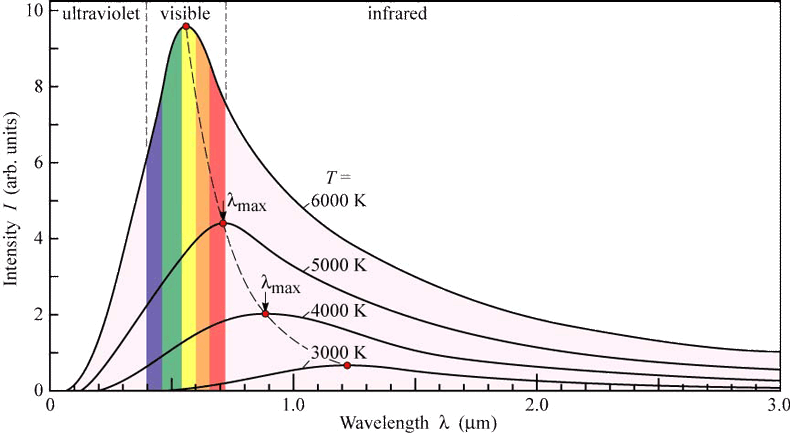
\includegraphics[width=0.75\linewidth]{figures/exampleFigure.png}
  \caption[Short Caption]{This is a long caption. It's too long  
         for the table of contents, so we specify a short caption 
         in the brackets.}
  \label{fig:IntensityVsWavelength}
\end{figure}
  \end{verbatim}
  \vspace{2mm}
\end{minipage}

Note the use of a short caption in brackets in the \texttt{\textbackslash caption} command.
This lets us have a long explanatory caption, without keeping our List of Tables compact (compare the caption of \cref{fig:IntensityVsWavelength}) with how it's listed on \cpageref{sec:ListOfTables}.

\begin{figure}
  \centering
  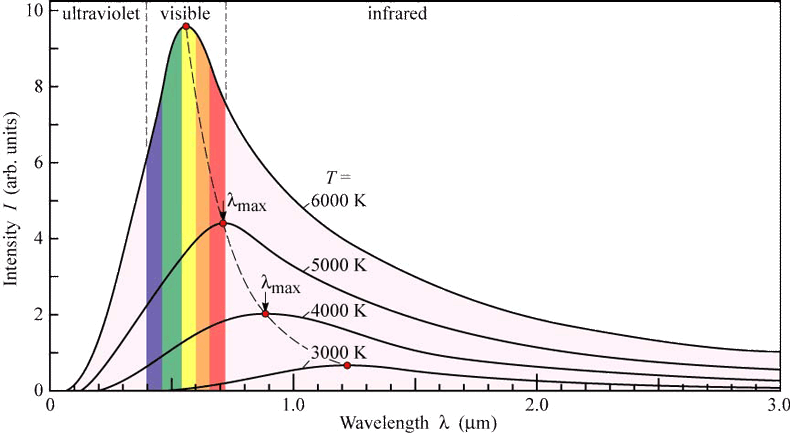
\includegraphics[width=0.75\linewidth]{figures/exampleFigure.png}
  \caption[Short Caption]{This is a long caption. It's too long  
         for the table of contents, so we specify a short caption 
         in the brackets.}
  \label{fig:IntensityVsWavelength}
\end{figure}

For large figures, it might be necessary to display it sideways (i.e., in landscape). 
If only the figure is to be done this way, the \texttt{\textbackslash sidewaysfigure} environment may be used:
\begin{verbatim}
  \begin{sidewaysfigure}
    \centering
    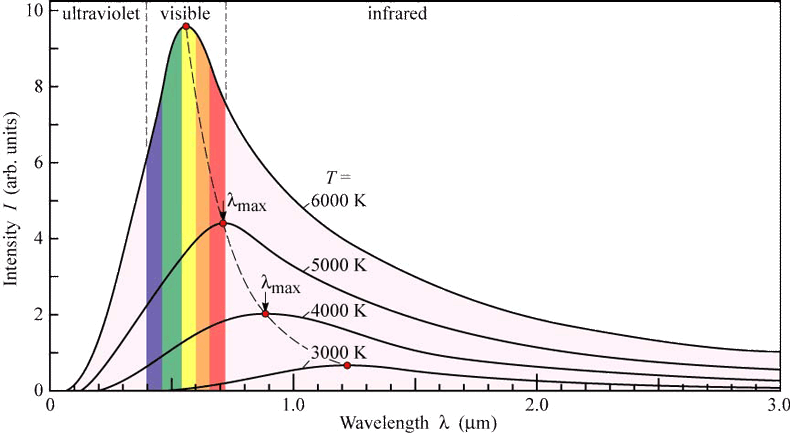
\includegraphics[width=0.5\textwidth]{figures/exampleFigure.png}
    \caption[Sideways Example Figure]{This is another example Figure, 
    rotated to landscape orientation.}
    \label{LandscapeFigure}
  \end{sidewaysfigure}
\end{verbatim}
The result of this code is shown in \cref{LandscapeFigure}. 
Note that this figure will occupy the entire page.
If you'd like to have landscape text as well, consider using the \texttt{lscape} or \texttt{pdflscape} packages.

  \begin{sidewaysfigure}
    \centering
    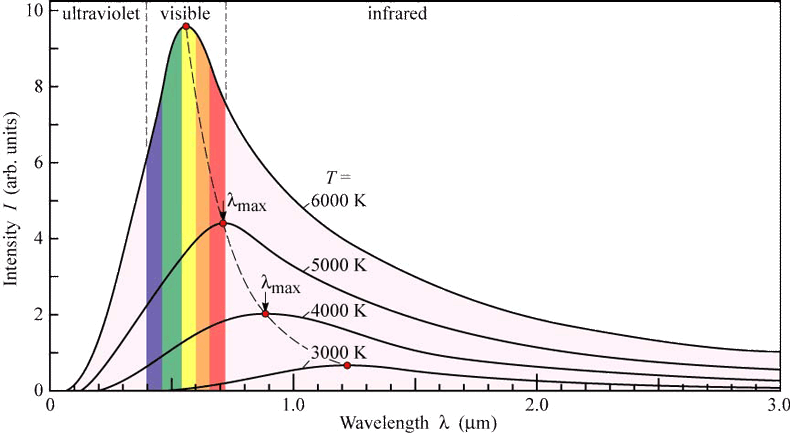
\includegraphics[width=0.5\textwidth]{figures/exampleFigure.png}
    \caption[Sideways Example Figure]{This is another example Figure, rotated to landscape orientation.}
    \label{LandscapeFigure}
  \end{sidewaysfigure}

\subsection{Math}

Math in \LaTeX{} is typeset in two ways: 
\begin{enumerate}
  \item \textbf{Display Mode} This is for equations that will appear on their own line, usually centered.
  Equations in display mode are typeset larger and have numbers by default.
  \item \textbf{Inline Mode} For symbols and short expressions that are to be displayed in running text.
\end{enumerate}

\subsubsection{Display Mode}
There are several environments for specifying display equations.
The original \TeX{} used \texttt{\$\$\,$\cdot$\,\$\$}, while \LaTeX{} uses \texttt{\textbackslash [\,$\cdot$\,\textbackslash ]}.
These still work, but \TeX{} primatives should be avoided (unless you know what you're doing) to avoid compatibility problems with newer packages.
If you're using \LaTeX{}, the \texttt{equation}, \texttt{eqnarray}, and \texttt{align} environments are your friends.
I recommend using the \texttt{align} environment exclusively for equations. 
It's virtually identical to \texttt{equation}, but allows you to have multiple lines and specify where you want them to---well---\emph{align} with each other using the \& character.
For example:
\begin{center}
\begin{minipage}{0.45\textwidth}
\vspace{2mm}
\small
\begin{verbatim}
\begin{align*}
  c &= \sqrt{ a^{2} + b^{2} } \\
  &= a\sqrt{1 + (a/b)^{2}}\,.
\end{align*}
\end{verbatim}
\end{minipage}~%
\begin{minipage}{0.45\textwidth}
\vspace{2mm}
\small
\begin{align*}
  c &= \sqrt{ a^{2} + b^{2} } \\
  &= a\sqrt{1 + (a/b)^{2}}\,.
\end{align*}
\end{minipage}
\end{center}

\subsubsection{Inline Mode}
For text that is to diplay inline, use \$$\,\cdot\,$\$.
For instance
\begin{center}
\begin{minipage}{0.45\textwidth}
\vspace{2mm}
\small
\begin{verbatim}
Here, $m$ is the mass, and 
$\ddot{x}$ is the acceleration.
\end{verbatim}
\end{minipage}~~~%
\begin{minipage}{0.45\textwidth}
\vspace{2mm}
\small
Here, $m$ is the mass, and $\ddot{x}$ is the acceleration.
\end{minipage}
\end{center}
While it is possible to typeset equations inline, this is sometimes a poor aesthetic choice, as it will cause the math to look a bit cramped and often alter the linespacing.
\begin{center}
\begin{minipage}{0.45\textwidth}
\vspace{1mm}
\scriptsize
\begin{verbatim}
The fundamental theorem says that
$\int_{a}^{b}{f(x)\,\mathrm{d}x}
= F(b) - F(a)$, though this is
really a special case of Stokes'
theorem, named for Irish physicist
George Stokes.
\end{verbatim}
\end{minipage}~~~%
\begin{minipage}{0.45\textwidth}
\vspace{1mm}
\small
The fundamental theorem says that
$\int_{a}^{b}{f(x)\,\mathrm{d}x}
= F(b) - F(a)$, though this is
really a special case of Stokes'
theorem, named for Irish physicist
George Stokes.
\end{minipage}
\end{center}

\subsection{Tables}
Tables are kind of a pain in \LaTeX.
There are some utilities that allow you to create a table and export the code, but I don't have much experience with these.
\Cref{tab:ValuesOfFunctions} shows a simple table; 
note that the caption must appear \emph{above} the table.
I do not like this convention, but there it is.

\begin{table}
\caption{This is an example Table.}
  \begin{center}
  \begin{tabular}{ccc}
    $x$ & $f(x)$ & $g(x)$ \\
    \hline
    1 & 6 & 4  \\
    2 & 6 & 3  \\
    3 & 6 & 2  \\
    4 & 6 & 2  \\
    \label{tab:ValuesOfFunctions}
  \end{tabular}
  \end{center}
\end{table}

\section{Cross-Referencing}
One of the chief advantages of \LaTeX{} is how easy it makes cross-references.
Sure, this can be done in Word, but if you've tried messing with field codes, you probably sensed that there was probably an easier way.
In this template items are referenced using \texttt{cleveref} and \texttt{hyperref} packages.
For example, suppose we type for an equation
{\small
\begin{verbatim}
\begin{align}
  i\hbar\frac{\partial}{\partial t}\psi 
  &=
  \left[ \frac{-\hbar^{2}}{2m}\nabla^{2} + V\right]\psi\,.
  \label{eqn:SchrodingerEquation}
\end{align}
\end{verbatim}
}%
which prints as
\begin{align}
  i\hbar\frac{\partial}{\partial t}\Psi &= \left[ \frac{-\hbar^{2}}{2m}\nabla^{2} + V\right]\Psi\,.
  \label{eqn:SchrodingerEquation}
\end{align}
To refer to this equationlater on, we type \verb|\cref{eqn:SchrodingerEquation}|, which prints as \cref{eqn:SchrodingerEquation}.

The \texttt{cleveref} package allows you to define how the refereces print out, e.g., Eq. 1 vs. eq.~(1); or Figure~1 vs. fig.~1, etc.
The \texttt{hyperef} package makes it so that all your references are clickable. 
So if you reference, for example, \cref{fig:IntensityVsWavelength} a few pages later, clicking it will jump back to the figure (try it).
Unfortunately there's no ``back'' button, so if you jump back, you have to manually scroll forward.

\section{Section}

\Blindtext

\subsection{Example Subsection}

\blindtext


\subsubsection{Example Subsubsection}

\blindtext

\section{God, \emph{Another} Section??? }

% This is a figure in landscape orientation

